\documentclass[10pt]{beamer}
\usepackage[utf8]{inputenc}
\usepackage[francais]{babel}
\usepackage[T1]{fontenc}
\usepackage[export]{adjustbox}
\newcommand\Fontvi{\fontsize{8}{7.2}\selectfont}

\usepackage{minted}
\usemintedstyle{colorful}
\usepackage{hyperref}
\hypersetup{
	colorlinks,
	citecolor=black,
	filecolor=black,
	linkcolor=black,
	urlcolor=blue
}

\usetheme{Frankfurt}
\usecolortheme{beaver}

\addtobeamertemplate{navigation symbols}{}{%
    \usebeamerfont{footline}%
    \usebeamercolor[fg]{footline}%
    \hspace{1em}%
    \insertframenumber/\inserttotalframenumber
}

\begin{document}
\logo{%
	\makebox[0.95\paperwidth]{%
		
\includegraphics[width=2.5cm,keepaspectratio]{images/hepia.jpg}%
		\hfill%
		
\includegraphics[width=2.5cm,keepaspectratio]{images/hesso.jpg}%
	}%
}

\title{BibApp Hepia}
\author{Steven Liatti}
\institute{Projet de semestre - Prof. Mickaël Hoerdt - Hepia ITI 3\up{ème} année}
\date{15 mars 2018}

\begin{frame}
\titlepage
\end{frame}

\begin{frame}
    \frametitle{Plan}
	\setcounter{tocdepth}{3}
	\tableofcontents
\end{frame}

\section{Introduction}
\subsection{Contexte}
\begin{frame}
	\frametitle{\secname}
	\framesubtitle{\subsecname}
    \begin{itemize}
        \item Bibliothèque se sert du réseau NEBIS
        \item Nouveautés et périodiques tous les mois
        \item Bibliothèque aimerait devenir plus attractive (manque de fréquentation)
    \end{itemize}
    \Large\textbf{Besoin : ajouter du contenu personnalisé}
\end{frame}

\subsection{Objectifs}
\begin{frame}
	\frametitle{\secname}
	\framesubtitle{\subsecname}
    \begin{itemize}
        \item Étude du framework Ionic (tuto + prototype)
        \item Architecture de l'application mobile/web (backend, frontend et interfaces)
        \item Réalisation de la base de données augmentée
        \begin{itemize}
            \item Basée sur les données de NEBIS
            \item Enrichie avec les données saisies par les bibliothécaires
            \item Accessible via le serveur REST avec mode utilisateur anonyme et authentifié
        \end{itemize}
        \item Design et implémentation des interfaces en collaboration avec les bibliothécaires
    \end{itemize}
\end{frame}

\section{Architecture}
\begin{frame}
	\frametitle{\secname}
	\begin{figure}
		\begin{center}
			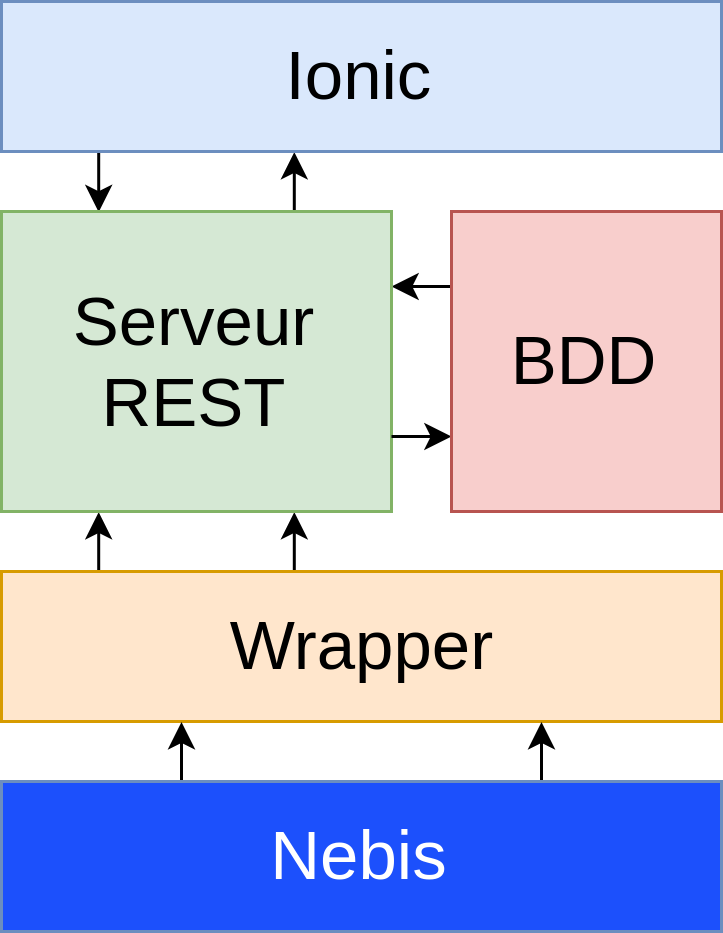
\includegraphics[width=0.5\textwidth]{images/architecture_final.png}
		\end{center}
	\end{figure}
\end{frame}

\section{Réalisation}
\subsection{Wrapper}
\begin{frame}
	\frametitle{\secname}
	\framesubtitle{\subsecname}
	\begin{itemize}
        \item Serveur Node.js
        \item Appels à l'API RIB NEBIS
        \item Trois routes, retournant des données en JSON :
        \begin{itemize}
            \item Liste des nouveautés pour année et mois donnés
            \item Recherche de documents selon certains critères
            \item Obtention des infos d'un ouvrage par ISBN ou ISSN
        \end{itemize}
    \end{itemize}
\end{frame}

\subsection{Serveur}
\begin{frame}
	\frametitle{\secname}
	\framesubtitle{\subsecname}
	\begin{itemize}
        \item Serveur Node.js
        \item Appels au Wrapper avec axios
        \item Authentification avec PassportJS, génération de JWT
        \item Routes GET, POST et DELETE pour gérer le contenu texte
        \item Gestion des images avec multer
    \end{itemize}
\end{frame}

\subsection{Base de données}
\begin{frame}
	\frametitle{\secname}
	\framesubtitle{\subsecname}
	\begin{columns}[T]
		\begin{column}{.5\textwidth}
            \begin{figure}
                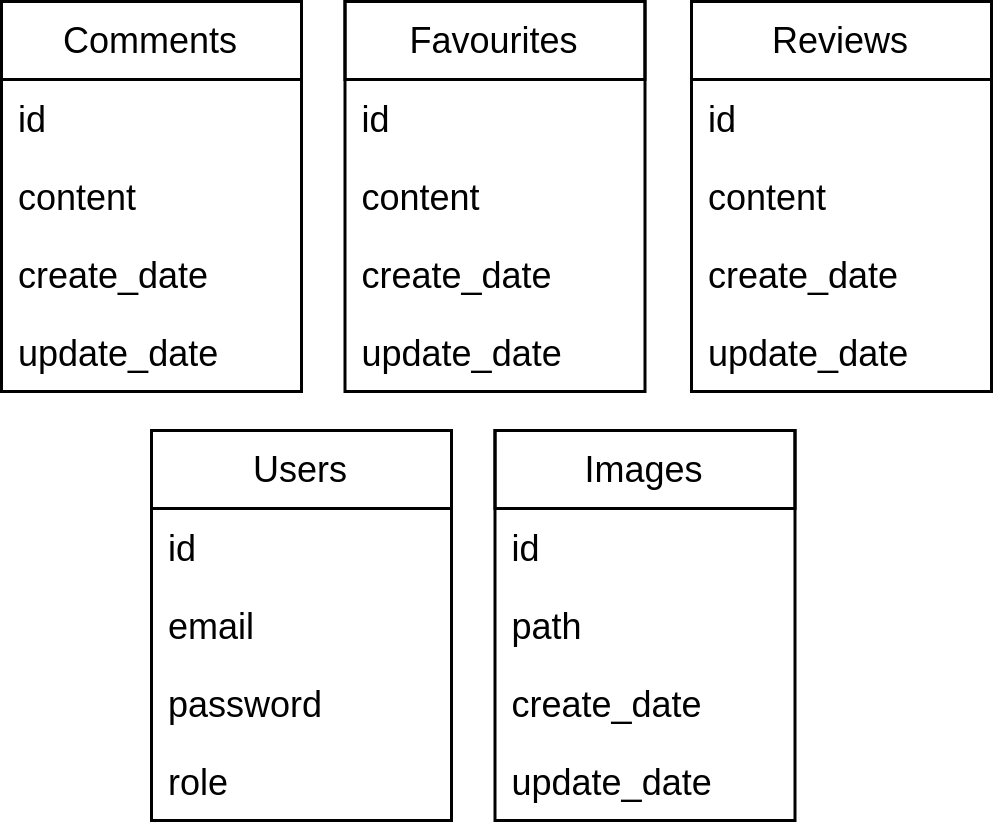
\includegraphics[width=1\textwidth]{images/bdd.png}
            \end{figure}
		\end{column}
		\begin{column}{.5\textwidth}
            \begin{itemize}
                \item Réalisée avec MongoDB et Mongoose (définition des schémas)
                \item Base de données augmentée, orientée documents
                \item Collections indépendantes, ISBN ou ISSN comme clé
            \end{itemize}
		\end{column}
	\end{columns}
\end{frame}

\subsection{Ionic}
\begin{frame}
	\frametitle{\secname}
	\framesubtitle{\subsecname (1)}
    \begin{itemize}
        \item Sections nouveautés, coups de coeur et revue de presse
        \item Page de détails pour un livre
        \item Pages de login et création de compte
        \item Champ de recherche
    \end{itemize}
\end{frame}

\begin{frame}
	\frametitle{\secname}
	\framesubtitle{\subsecname (2)}
    \begin{columns}[T]
        \begin{column}{.3\textwidth}
            \begin{figure}
                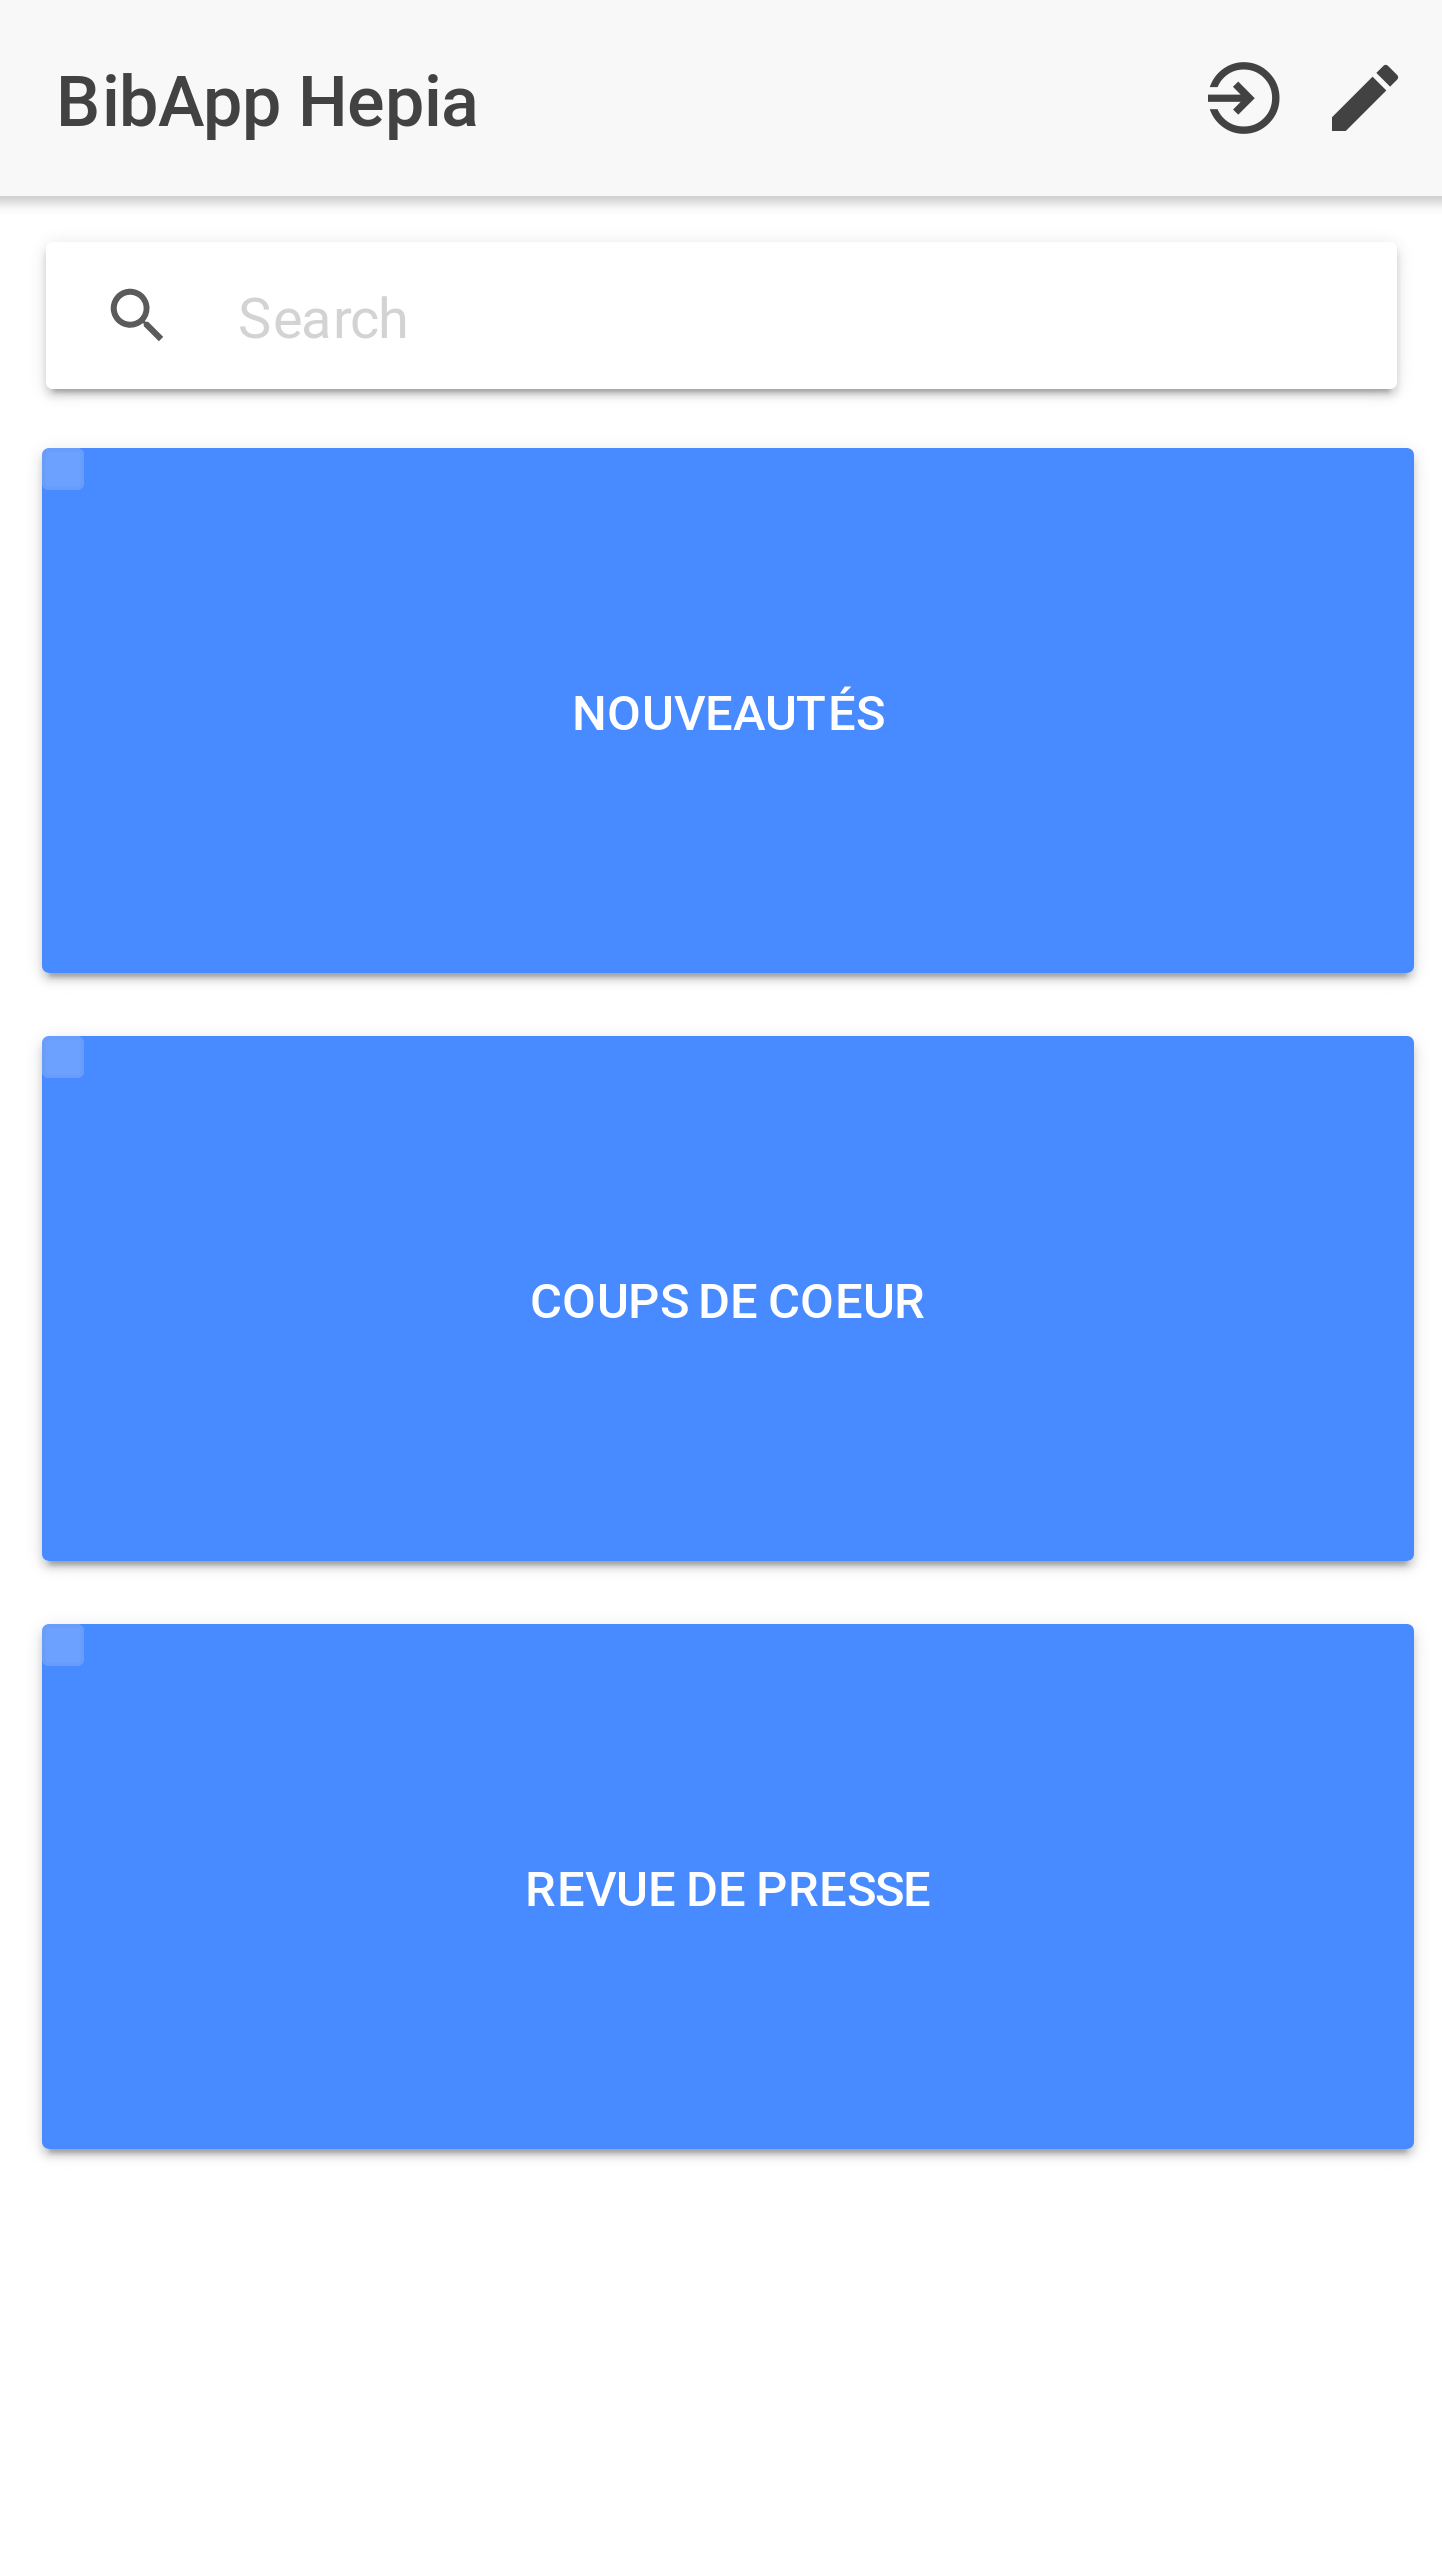
\includegraphics[width=1\textwidth]{images/screenshots/android1.png}
            \end{figure}
        \end{column}
        \begin{column}{.3\textwidth}
            \begin{figure}
                
\includegraphics[width=1\textwidth]{images/screenshots/android3.png}
            \end{figure}
        \end{column}
        \begin{column}{.3\textwidth}
            \begin{figure}
                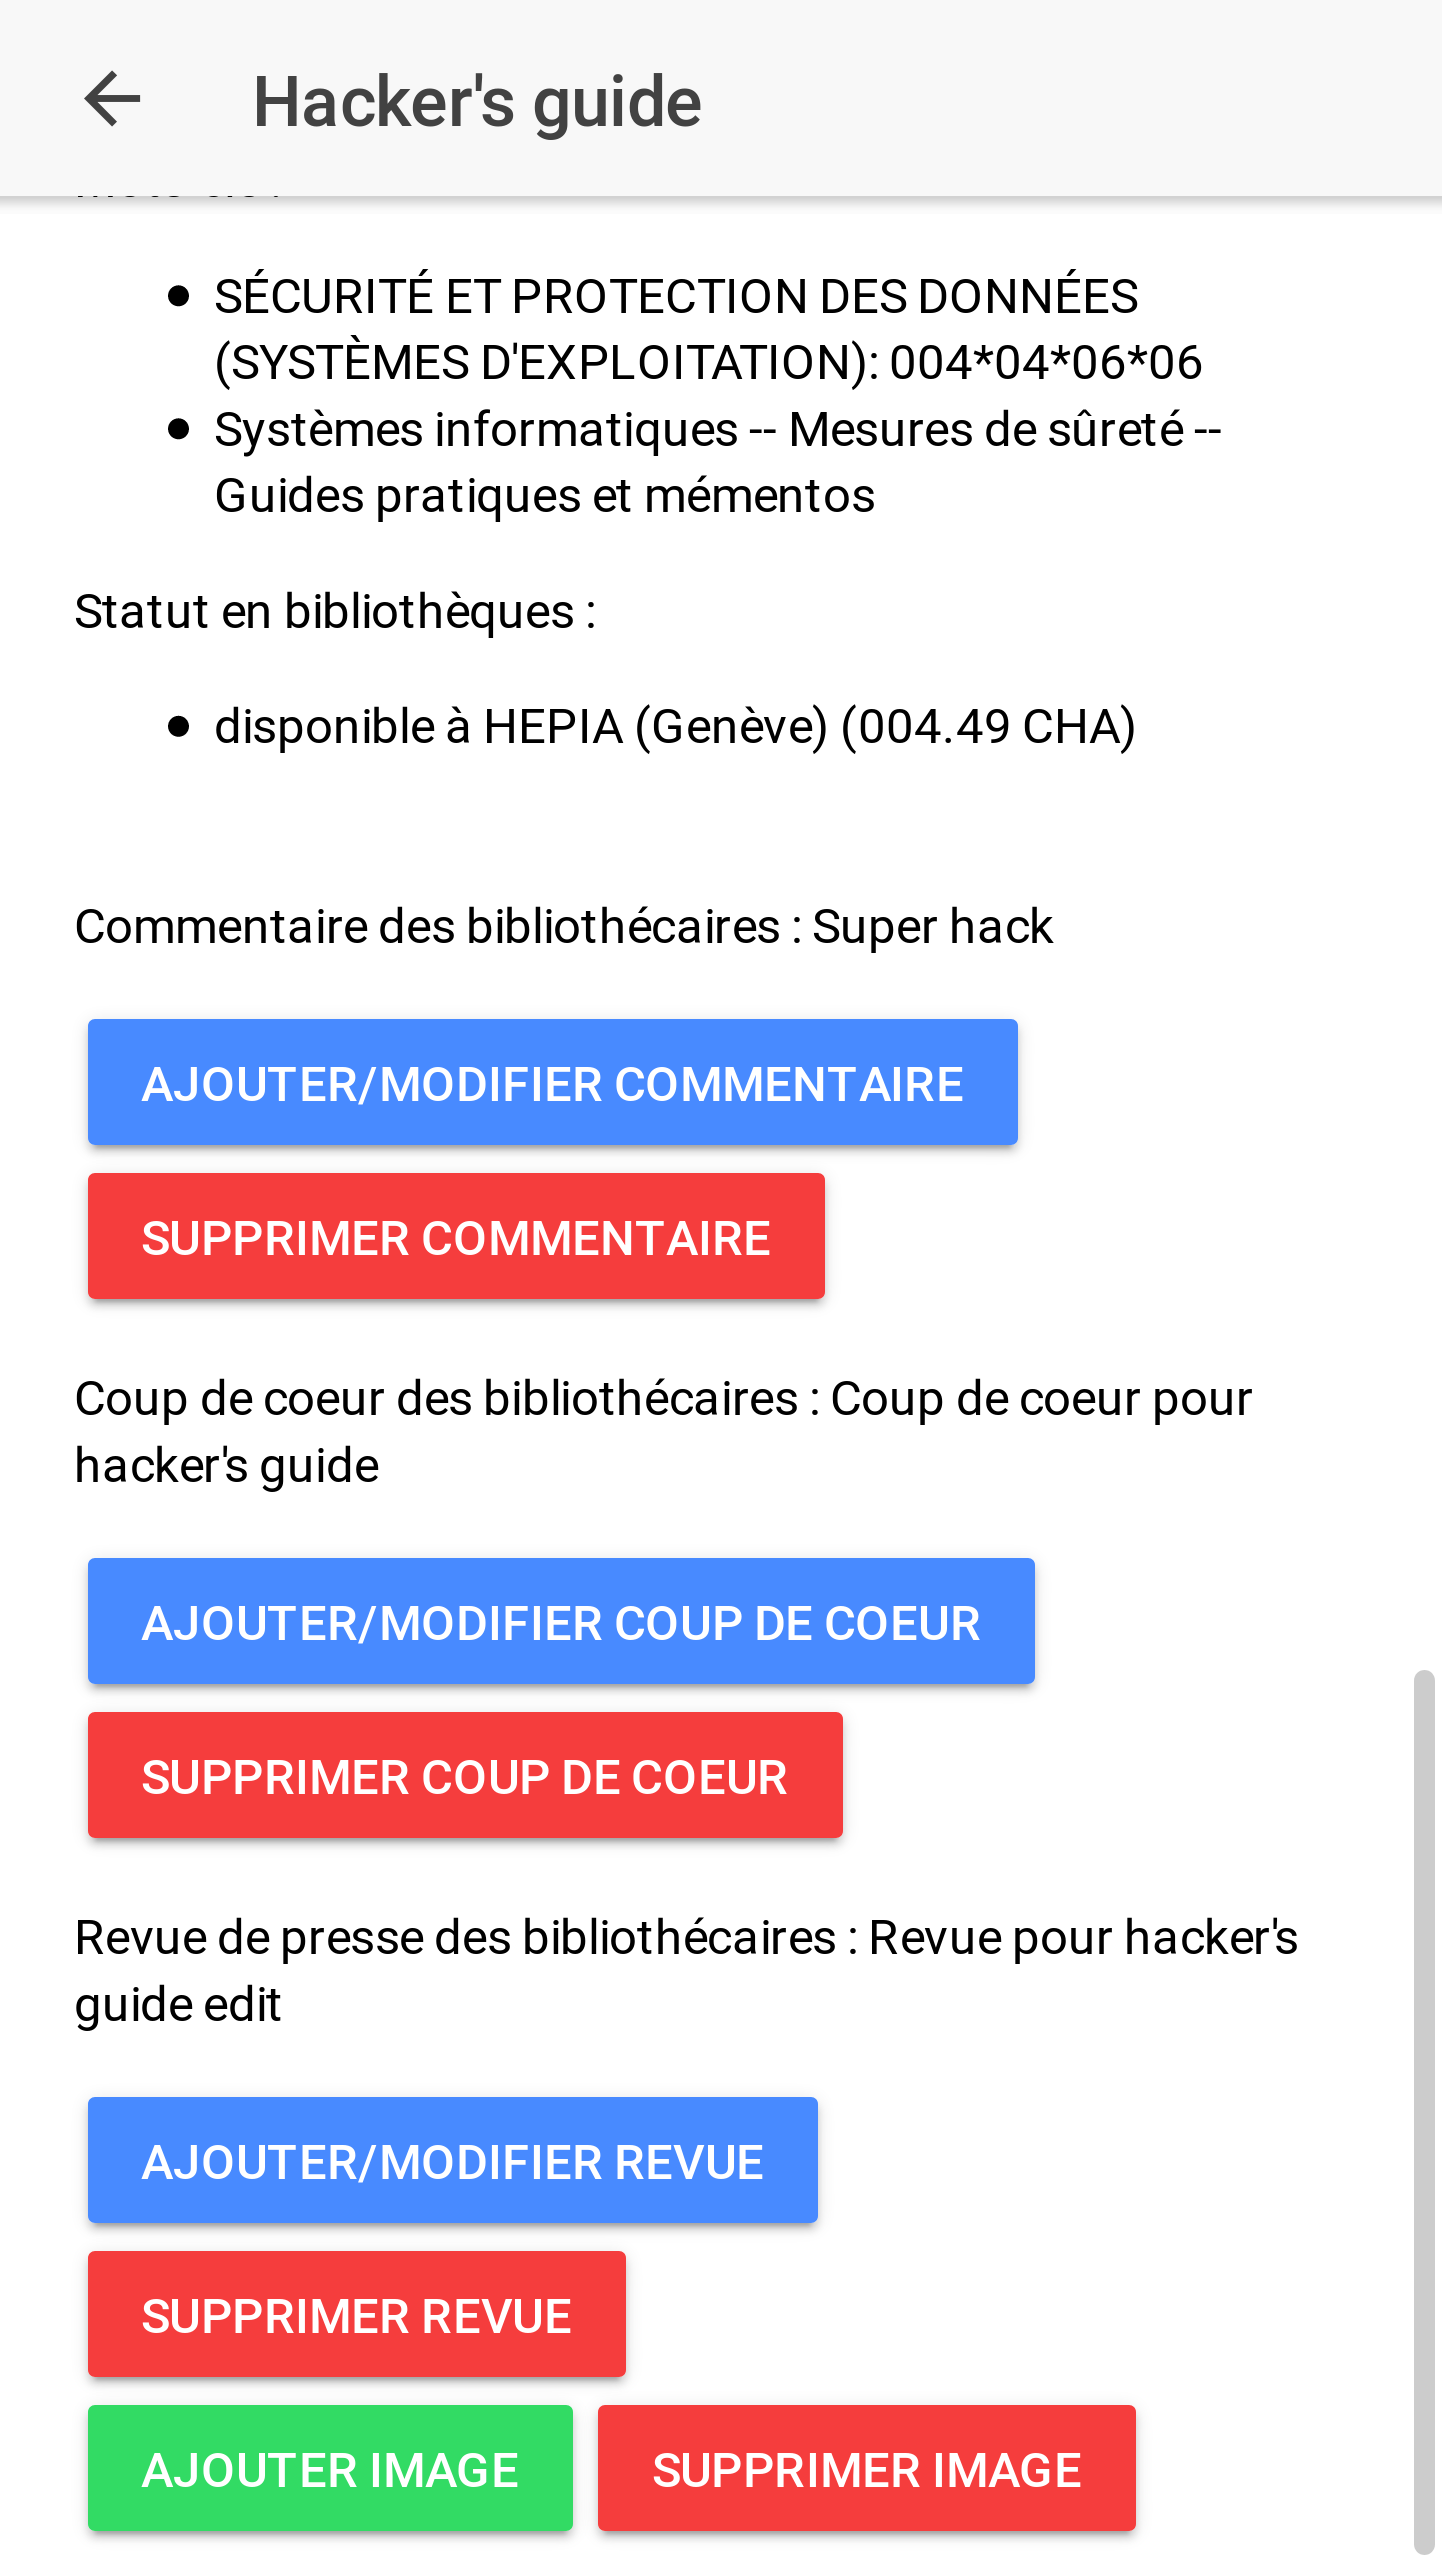
\includegraphics[width=1\textwidth]{images/screenshots/android7.png}
            \end{figure}
        \end{column}
    \end{columns}
\end{frame}

\section{Conclusion}
\begin{frame}
	\frametitle{\secname}
	\begin{itemize}
        \item Perfectionnement de mes compétences en développement web
        \item Découverte du framework Ionic
        \item Améliorations :
        \begin{itemize}
            \item Préférer une interface d'administration dédiée pour l'ajout de contenu
            \item Amélioration de l'expérience utilisateur sur l'app Ionic
        \end{itemize}
    \end{itemize}
\end{frame}

\end{document}
